%!TEX TS-program = xelatex
\documentclass[12pt, a4paper, oneside]{article}

% пакеты для математики
\usepackage{amsmath,amsfonts,amssymb,amsthm,mathtools}  
\mathtoolsset{showonlyrefs=true}  % Показывать номера только у тех формул, на которые есть \eqref{} в тексте.

\usepackage[english, russian]{babel} % выбор языка для документа
% \usepackage[utf8]{inputenc}          % utf8 кодировка

% Основные шрифты 
\usepackage{fontspec}         
\setmainfont{Linux Libertine O}  % задаёт основной шрифт документа

% Математические шрифты 
\usepackage{unicode-math}     
\setmathfont[math-style=upright]{[Neo Euler.otf]} 


%%%%%%%%%% Работа с картинками и таблицами %%%%%%%%%%
\usepackage{graphicx} % Для вставки рисунков                
\usepackage{graphics}
\graphicspath{{images/}{pictures/}}   % папки с картинками

\usepackage{wrapfig}    % обтекание рисунков и таблиц текстом

\usepackage{booktabs}   % таблицы как в годных книгах
\usepackage{tabularx}   % новые типы колонок
\usepackage{tabulary}   % и ещё новые типы колонок
\usepackage{float}      % возможность позиционировать объекты в нужном месте
\renewcommand{\arraystretch}{1.2}  % больше расстояние между строками


%%%%%%%%%% Графики и рисование %%%%%%%%%%
\usepackage{tikz, pgfplots}  % языки для графики
\pgfplotsset{compat=1.16}

\usepackage{todonotes} % для вставки в документ заметок о том, что осталось сделать
% \todo{Здесь надо коэффициенты исправить}
% \missingfigure{Здесь будет Последний день Помпеи}
% \listoftodos --- печатает все поставленные \todo'шки


%%%%%%%%%% Внешний вид страницы %%%%%%%%%%

\usepackage[paper=a4paper, top=20mm, bottom=15mm,left=20mm,right=15mm]{geometry}
\usepackage{indentfirst}    % установка отступа в первом абзаце главы

\usepackage{setspace}
\setstretch{1.15}  % межстрочный интервал
\setlength{\parskip}{4mm}   % Расстояние между абзацами
% Разные длины в LaTeX: https://en.wikibooks.org/wiki/LaTeX/Lengths

% свешиваем пунктуацию
% теперь знаки пунктуации могут вылезать за правую границу текста, при этом текст выглядит ровнее
\usepackage{microtype}

% \flushbottom                            % Эта команда заставляет LaTeX чуть растягивать строки, чтобы получить идеально прямоугольную страницу
\righthyphenmin=2                       % Разрешение переноса двух и более символов
\widowpenalty=300                     % Небольшое наказание за вдовствующую строку (одна строка абзаца на этой странице, остальное --- на следующей)
\clubpenalty=3000                     % Приличное наказание за сиротствующую строку (омерзительно висящая одинокая строка в начале страницы)
\tolerance=10000     % Ещё какое-то наказание.

% мои цвета https://www.artlebedev.ru/colors/
\definecolor{titleblue}{rgb}{0.2,0.4,0.6} 
\definecolor{blue}{rgb}{0.2,0.4,0.6} 
\definecolor{red}{rgb}{1,0,0.2} 
\definecolor{green}{rgb}{0,0.6,0} 
\definecolor{purp}{rgb}{0.4,0,0.8} 

% цвета из geogebra 
\definecolor{litebrown}{rgb}{0.6,0.2,0}
\definecolor{darkbrown}{rgb}{0.75,0.75,0.75}

% Гиперссылки
\usepackage{xcolor}   % разные цвета

\usepackage{hyperref}
\hypersetup{
	unicode=true,           % позволяет использовать юникодные символы
	colorlinks=true,       	% true - цветные ссылки
	urlcolor=blue,          % цвет ссылки на url
	linkcolor=red,          % внутренние ссылки
	citecolor=green,        % на библиографию
	breaklinks              % если ссылка не умещается в одну строку, разбивать её на две части?
}

% меняю оформление секций 
\usepackage{titlesec}
\usepackage{sectsty}

% меняю цвет на синий
\sectionfont{\color{titleblue}}
\subsectionfont{\color{titleblue}}

% выбрасываю нумерацию страниц и колонтитулы 
\pagestyle{empty}

% синие круглые бульпоинты в списках itemize 
\usepackage{enumitem}

\definecolor{itemizeblue}{rgb}{0, 0.45, 0.70}

\newcommand*{\MyPoint}{\tikz \draw [baseline, fill=itemizeblue, draw=blue] circle (2.5pt);}

\renewcommand{\labelitemi}{\MyPoint}

% расстояние в списках
\setlist[itemize]{parsep=0.4em,itemsep=0em,topsep=0ex}
\setlist[enumerate]{parsep=0.4em,itemsep=0em,topsep=0ex}


%%%%%%%%%% Свои команды %%%%%%%%%%

% Математические операторы первой необходимости:
\DeclareMathOperator{\sgn}{sign}
\DeclareMathOperator*{\argmin}{arg\,min}
\DeclareMathOperator*{\argmax}{arg\,max}
\DeclareMathOperator{\Cov}{Cov}
\DeclareMathOperator{\Var}{Var}
\DeclareMathOperator{\Corr}{Corr}
\DeclareMathOperator{\E}{\mathop{E}}
\DeclareMathOperator{\Med}{Med}
\DeclareMathOperator{\Mod}{Mod}
\DeclareMathOperator*{\plim}{plim}

% команды пореже
\newcommand{\const}{\mathrm{const}}  % const прямым начертанием
\newcommand{\iid}{\sim i.\,i.\,d.}  % ну вы поняли...
\newcommand{\fr}[2]{\ensuremath{^{#1}/_{#2}}}   % особая дробь
\newcommand{\ind}[1]{\mathbbm{1}_{\{#1\}}} % Индикатор события
\newcommand{\dx}[1]{\,\mathrm{d}#1} % для интеграла: маленький отступ и прямая d

% одеваем шапки на частые штуки
\def \hb{\hat{\beta}}
\def \hs{\hat{s}}
\def \hy{\hat{y}}
\def \hY{\hat{Y}}
\def \he{\hat{\varepsilon}}
\def \hVar{\widehat{\Var}}
\def \hCorr{\widehat{\Corr}}
\def \hCov{\widehat{\Cov}}

% Греческие буквы
\def \a{\alpha}
\def \b{\beta}
\def \t{\tau}
\def \dt{\delta}
\def \e{\varepsilon}
\def \ga{\gamma}
\def \kp{\varkappa}
\def \la{\lambda}
\def \sg{\sigma}
\def \tt{\theta}
\def \Dt{\Delta}
\def \La{\Lambda}
\def \Sg{\Sigma}
\def \Tt{\Theta}
\def \Om{\Omega}
\def \om{\omega}

% Готика
\def \mA{\mathcal{A}}
\def \mB{\mathcal{B}}
\def \mC{\mathcal{C}}
\def \mE{\mathcal{E}}
\def \mF{\mathcal{F}}
\def \mH{\mathcal{H}}
\def \mL{\mathcal{L}}
\def \mN{\mathcal{N}}
\def \mU{\mathcal{U}}
\def \mV{\mathcal{V}}
\def \mW{\mathcal{W}}

% Жирные буквы
\def \mbb{\mathbb}
\def \RR{\mbb R}
\def \NN{\mbb N}
\def \ZZ{\mbb Z}
\def \PP{\mbb{P}}
\def \QQ{\mbb Q}


%%%%%%%%%% Теоремы %%%%%%%%%%
\theoremstyle{plain} % Это стиль по умолчанию.  Есть другие стили.
\newtheorem{theorem}{Теорема}[section]
\newtheorem{result}{Следствие}[theorem]
% счётчик подчиняется теоремному, нумерация идёт по главам согласованно между собой

% убирает курсив и что-то еще наверное делает ;)
\theoremstyle{definition}         
\newtheorem*{definition}{Определение}  % нумерация не идёт вообще


%%%%%%%%%% Задачки и решения %%%%%%%%%%
\usepackage{etoolbox}    % логические операторы для своих макросов
\usepackage{environ}
\newtoggle{lecture}

\newcounter{problem}%[section]  % счётчик для упражнений 

\renewcommand{\theproblem}{\arabic{problem}}

\newenvironment{problem}[1]{
\addtocounter{problem}{1}\noindent{ \color{titleblue} \large \bfseries Упражнение~\theproblem~#1 \vspace{1ex} \newline}
}{ }

% Окружение, чтобы можно было убирать решения из pdf
\NewEnviron{solution}{%
  \iftoggle{lecture}
    {\noindent \textbf{\large Решение:} \vspace{1ex} \newline \BODY}
    {}%
  }
  
% выделение по тексту важных вещей
\newcommand{\indef}[1]{\textbf{ \color{green} #1}} 

\begin{document} % Конец преамбулы, начало файла

% Если переключить в false, все solution исчезнут из pdf
\toggletrue{lecture}
%\togglefalse{lecture}

% эпиграфы
\usepackage{epigraph}
\setlength\epigraphwidth{.4\textwidth}
\setlength\epigraphrule{0pt}


\section*{Семинар 11: Введение в АБ-тесты}

\epigraph{Безумная цитата}{автор этой цитаты}

На этом семинаре разговор пойдёт про АБ-тесты и проверку гипотез. Задачки из этого семинара призваны просто продемонстрировать откуда растут ноги всей замысловатой процедуры с проверкой гипотезы. Из-за этого понятия в задачках иногда формулируются не очень чётко. Если вы хотите уметь профессионально проверять гипотезы, а не просто иметь об этом какое-то представление, лучше почитайте учебник. 

\begin{problem}{(которое сеет в наших головах раздор и сомнение)}
В Селе  АБтестово проживает $4$ человека. У каждого из них свой рост:

\begin{center}
	\begin{tabular}{lc}
		\toprule
		Маша &  $150$\\
		Паша &  $160$\\
		Саша &  $180$\\
		Даша &  $190$\\ 
		\bottomrule
	\end{tabular}	
\end{center}

Дедя Фёдор, Шарик и Матроскин проезжают через АБтестово в Простоквашино транзитом. Каждый из них заинтересовался ростом местных жителей и решил по небольшой подвыборке из двух человек посчитать средний рост всех жителей АБтестово. 

\begin{enumerate} 
	\item[а)] Посчитайте настоящий средний рост в АБтестово по всей генеральной совокупности.
	\item[б)] Шарик посчитал средние по Саше и Даше и сказал, что это оценка среднего роста в АБ-тестово. Сколько у него получилось? Насколько сильно эта оценка отличается от настоящего среднего? 
	\item[в)] К Матроскину в выборку затесались Маша и Паша. Какую оценку он получил? Далека ли она от реального среднего? 
	\item[г)] К дяде Фёдору в выборку попали Маша и Саша. Как дела обстоят с его оценкой? 
	\item[д)] Подерутся ли между собой Шарик, Матроскин и дядя Фёдор? Почему результаты получились именно такими? Может ли так происходить в реальности? 
\end{enumerate} 
\end{problem}

\begin{solution}
Давайте вспоминать семинар по матстату, который мы с вами не так давно решали. Подсчитаем средний рост в АБтестово  по всей генеральной совокупности: 

\[
\frac{1}{4} \cdot (190 + 180 + 160 + 150) = 170.
\]

Посчитаем такие же средние по маленьким выборкам, которые собрали ребята: 

\begin{equation*} 
\begin{aligned} 
& \text{Фёдор:}  & 0.5 \cdot (190 + 150) = 170 \\
& \text{Шарик:}  & 0.5 \cdot (190 + 180) = 185 \\
& \text{Матроскин:} & 0.5 \cdot (150 + 160) = 155 
\end{aligned}
\end{equation*}

Видим, что значения у выборочных средних получились очень разными. При этом расстояние от среднего Шарика до настоящего равно $15$, от среднего Матроскина тоже $15$. От среднего Фёдора до настоящего нулевое. 

Каждый житель Простоквашино посчитал средний рост по двум жителям АБтестово. У дяди Фёдора результат совпал с настоящим средним. Означает ли это, что он оценивал среднее правильнее своих коллег?  \indef{На самом деле нет. Ему просто повезло.}  Из-за того, что отбор людей в выборку происходит случайно, средний рост оказывается случайной величиной с распределением, которое мы построим в следующей задачке. Если бы жители Простоквашино понимали это, они бы не подрались. А так, конечно, передерутся. 

Происходят ли такие ситуации в реальности? Да сплошь и рядом. Каждая характеристика (среднее, доля и тп), которую мы пытаемся оценить, чтобы проверить какой-то эффект (вырастут ли продажи, если поменять дизайн бутылки) или ответить на давно мучающий нас вопрос (правда ли, что в Австралии зарплаты у девушек выше, чем у мужчин, то есть девушек дискриминируют), считается по случайной выборке из генеральной совокупности. \indef{Любая выборочная характеристика будет случайной величиной.} Из-за этого нам нужно придумать какой-то способ работать с такими характеристиками, чтобы несмотря на случайность выборки, почти не ошибаться. 
\end{solution}


\begin{problem}{(в котором происходит исследование)}
Жизнь в Простоквашино изрядно испортилась. Почтальону Печкину надоела вся эта ругань. Чтобы раз и навсегда покончить с раздорами, он сел на велосипед и поехал в АБтестово. Там он опросил всех четверых жителей села, а после стал фантазировать что могло бы получиться в качестве среднего, если бы он опросил только двух каких-то жителей. 

\begin{enumerate} 
	\item[а)] Является ли средний рост случайной величиной? Сколько значений принимает эта случайная величина (сколько вариантов опросить местных жителей есть у Печкина)?
	\item[б)] Найдите все возможные значения среднего роста в АБтестово. Постройте гистограмму для этого среднего значения. Как и в прошлый раз, столбики стройте с шагом $5$, верхнюю границу включайте в столбик. Отметьте на картинке рост, который получил Шарик, дядя Фёдор и Матроскин. Какая из оценок ближе всего к центру распределения? 
	\item[в)] Какова вероятность оказаться в хвостах распределения? Какова вероятность оказаться в его центре? 
\end{enumerate} 
\end{problem}

\begin{solution}
Да. Средний рост --- случайная величина. Если вы немного помните со школы комбинаторику, вы можете посчитать сколько значений она принимает. Это число сочетаний из $4$ по $2$:  $C_4^2 = \frac{4!}{2!2!} =  6$. Если не помните, вы можете в явном виде перечислить все пары жителей. Но комбинаторику я бы на вашем месте повторил. Это полезно --- уметь считать количество разных комбинаций\footnote{Вот хорошая и простая книга (Виленкин, Комбинаторика): \url{https://yadi.sk/i/X1Cvq8hMdTSHQA}}.  

Давайте выпишем все значения, которые может принять средний рост: 

\begin{equation*}
\begin{aligned}
& \text{Маша и Паша}  & 0.5 \cdot (150 + 160) = 155 \\
& \text{Маша и Cаша}  & 0.5 \cdot (150 + 190) = 170 \\
& \text{Маша и Даша}  & 0.5 \cdot (150 + 180) = 165 \\
& \text{Паша и Саша}  & 0.5 \cdot (160 + 190) = 175 \\
& \text{Паша и Даша}  & 0.5 \cdot (160 + 180) =  170 \\
& \text{Саша и Даша}  & 0.5 \cdot (190 + 180) =  185 \\
\end{aligned} 
\end{equation*}

Каждое из этих значений случайная величина принимает равновероятно, так как мы берём двух человек из генеральной совокупности абсолютно случайно.  Давайте нарисуем гистограмму для этого распределений. 

\begin{center}
\definecolor{zzttqq}{rgb}{0.6,0.2,0.}
\definecolor{cqcqcq}{rgb}{0.75,0.75,0.75}
\begin{tikzpicture}[line cap=round,line join=round,x=1.0cm,y=1.0cm]
\draw [color=cqcqcq,, xstep=1.0cm,ystep=1.0cm] (-3.2,-0.18) grid (6.3,6.12);
\clip(-3.2,-0.18) rectangle (6.3,6.12);
\fill[line width=2.pt,color=zzttqq,fill=zzttqq,fill opacity=0.10000000149011612] (-1.,1.) -- (-1.,2.) -- (-0.5,2) -- (-0.5,1.) -- cycle;
\fill[line width=2.pt,color=zzttqq,fill=zzttqq,fill opacity=0.10000000149011612] (1.5,1.) -- (1.5,2) -- (2.,2.) -- (2.,1.) -- cycle;
\fill[line width=2.pt,color=zzttqq,fill=zzttqq,fill opacity=0.10000000149011612] (2.,1.) -- (2.,3.) -- (2.5,3) -- (2.5,1.) -- cycle;
\fill[line width=2.pt,color=zzttqq,fill=zzttqq,fill opacity=0.10000000149011612] (2.5,1.) -- (2.5,2) -- (3.,2.) -- (3.,1.) -- cycle;
\fill[line width=2.pt,color=zzttqq,fill=zzttqq,fill opacity=0.10000000149011612] (4.,1.) -- (4.,2.) -- (4.5,2) -- (4.5,1) -- cycle;
\draw [->,line width=2.pt] (-3.,1.) -- (6.,1.);
\draw [->,line width=2.pt] (-2.,0.38) -- (-2.,5.);
\draw [line width=2.pt,color=zzttqq] (-1.,1.)-- (-1.,2.);
\draw [line width=2.pt,color=zzttqq] (-1.,2.)-- (-0.5,2);
\draw [line width=2.pt,color=zzttqq] (-0.5,2)-- (-0.5,1.);
\draw [line width=2.pt,color=zzttqq] (-0.5,1.)-- (-1.,1.);
\draw [line width=2.pt,color=zzttqq] (1.5,1.)-- (1.5,2);
\draw [line width=2.pt,color=zzttqq] (1.5,2)-- (2.,2.);
\draw [line width=2.pt,color=zzttqq] (2.,2.)-- (2.,1.);
\draw [line width=2.pt,color=zzttqq] (2.,1.)-- (1.5,1.);
\draw [line width=2.pt,color=zzttqq] (2.,1.)-- (2.,3.);
\draw [line width=2.pt,color=zzttqq] (2.,3.)-- (2.5,3);
\draw [line width=2.pt,color=zzttqq] (2.5,3)-- (2.5,1.);
\draw [line width=2.pt,color=zzttqq] (2.5,1.)-- (2.,1.);
\draw [line width=2.pt,color=zzttqq] (2.5,1.)-- (2.5,2);
\draw [line width=2.pt,color=zzttqq] (2.5,2)-- (3.,2.);
\draw [line width=2.pt,color=zzttqq] (3.,2.)-- (3.,1.);
\draw [line width=2.pt,color=zzttqq] (3.,1.)-- (2.5,1.);
\draw [line width=2.pt,color=zzttqq] (4.,1.)-- (4.,2.);
\draw [line width=2.pt,color=zzttqq] (4.,2.)-- (4.5,2);
\draw [line width=2.pt,color=zzttqq] (4,1)-- (4.5,1);
\draw [line width=2.pt,color=zzttqq] (4.5,1)-- (4.5,2.);
\draw (-0.8,1) node[anchor=north west] {$155$};
\draw (1.5,1) node[anchor=north west] {$165$};
\draw (4,1) node[anchor=north west] {$185$};
\end{tikzpicture}
\end{center}

Отметим на гистограмме точки Фёдора, Шарика и Матроскина: 

\begin{center}
	\definecolor{zzttqq}{rgb}{0.6,0.2,0.}
	\definecolor{cqcqcq}{rgb}{0.75,0.75,0.75}
	\definecolor{ududff}{rgb}{0.3,0.3,1.}
	\begin{tikzpicture}[line cap=round,line join=round,x=1.0cm,y=1.0cm]
	\draw [color=cqcqcq,, xstep=1.0cm,ystep=1.0cm] (-3.2,-0.18) grid (6.3,6.12);
	\clip(-3.2,-0.18) rectangle (6.3,6.12);
	\fill[line width=2.pt,color=zzttqq,fill=zzttqq,fill opacity=0.10000000149011612] (-1.,1.) -- (-1.,2.) -- (-0.5,2) -- (-0.5,1.) -- cycle;
	\fill[line width=2.pt,color=zzttqq,fill=zzttqq,fill opacity=0.10000000149011612] (1.5,1.) -- (1.5,2) -- (2.,2.) -- (2.,1.) -- cycle;
	\fill[line width=2.pt,color=zzttqq,fill=zzttqq,fill opacity=0.10000000149011612] (2.,1.) -- (2.,3.) -- (2.5,3) -- (2.5,1.) -- cycle;
	\fill[line width=2.pt,color=zzttqq,fill=zzttqq,fill opacity=0.10000000149011612] (2.5,1.) -- (2.5,2) -- (3.,2.) -- (3.,1.) -- cycle;
	\fill[line width=2.pt,color=zzttqq,fill=zzttqq,fill opacity=0.10000000149011612] (4.,1.) -- (4.,2.) -- (4.5,2) -- (4.5,1) -- cycle;
	\draw [->,line width=2.pt] (-3.,1.) -- (6.,1.);
	\draw [->,line width=2.pt] (-2.,0.38) -- (-2.,5.);
	\draw [line width=2.pt,color=zzttqq] (-1.,1.)-- (-1.,2.);
	\draw [line width=2.pt,color=zzttqq] (-1.,2.)-- (-0.5,2);
	\draw [line width=2.pt,color=zzttqq] (-0.5,2)-- (-0.5,1.);
	\draw [line width=2.pt,color=zzttqq] (-0.5,1.)-- (-1.,1.);
	\draw [line width=2.pt,color=zzttqq] (1.5,1.)-- (1.5,2);
	\draw [line width=2.pt,color=zzttqq] (1.5,2)-- (2.,2.);
	\draw [line width=2.pt,color=zzttqq] (2.,2.)-- (2.,1.);
	\draw [line width=2.pt,color=zzttqq] (2.,1.)-- (1.5,1.);
	\draw [line width=2.pt,color=zzttqq] (2.,1.)-- (2.,3.);
	\draw [line width=2.pt,color=zzttqq] (2.,3.)-- (2.5,3);
	\draw [line width=2.pt,color=zzttqq] (2.5,3)-- (2.5,1.);
	\draw [line width=2.pt,color=zzttqq] (2.5,1.)-- (2.,1.);
	\draw [line width=2.pt,color=zzttqq] (2.5,1.)-- (2.5,2);
	\draw [line width=2.pt,color=zzttqq] (2.5,2)-- (3.,2.);
	\draw [line width=2.pt,color=zzttqq] (3.,2.)-- (3.,1.);
	\draw [line width=2.pt,color=zzttqq] (3.,1.)-- (2.5,1.);
	\draw [line width=2.pt,color=zzttqq] (4.,1.)-- (4.,2.);
	\draw [line width=2.pt,color=zzttqq] (4.,2.)-- (4.5,2);
	\draw [line width=2.pt,color=zzttqq] (4,1)-- (4.5,1);
	\draw [line width=2.pt,color=zzttqq] (4.5,1)-- (4.5,2.);
	\draw [fill=ududff] (-0.5,1) circle (3pt);
	\draw (-0.8,1) node[anchor=north west] {$155$};
	\draw [fill=ududff] (2.5,1) circle (3pt);
	\draw (2.5,1) node[anchor=north west] {$170$};
	\draw [fill=ududff] (4.5,1) circle (3pt);
	\draw (4,1) node[anchor=north west] {$185$};	
	\end{tikzpicture}
\end{center}

Что мы видим? Мы видим, что Шарик и Матроскин своими оценками попали в хвосты распределения. То есть им очень не повезло.  Вероятность попасть в хвосты равна $\frac{2}{6} = \frac{1}{3}$. Оценка дяди Фёдора находится в центре распределения, и из-за этого является адекватной. 
\end{solution}


\begin{problem}{(в котором вскрывается правда)}
Построив распределение для среднего значения роста в АБтестово, Печкин очень сильно удивился. Оказалось, что это случайная величина. Печкин решил узнать у своего друга по переписке, Роналда Фишера, как правильно делать выводы, когда ты видишь только \indef{часть генеральной совокупности, то есть выборку.}

Фишер объяснил Печкину, что $\bar x$ при большом числе наблюдений, вошедших в него, имеет нормальное распределение. Когда мы хотим сделать выводы о среднем, нам нужно работать сразу со всем распределением. Например, с помощью правила трёх сигм для него можно построить доверительный интервал, то есть интервал, в котором с вероятностью $99\%$ лежит истинное значение среднего.  

\begin{enumerate}
	\item[а)] Найдите стандартное отклонение для Шарика, Матроскина и Фёдора по формуле 
	
	\[\hat \sigma = \sqrt{ \frac{1}{n-1}  \sum (x_i - \bar x)^2}.\]
	
	\item[б)] Постройте для каждого из парней доверительный интервал по правилу трёх сигм. Обратите внимание, что стандартное отклонение, которое мы посчитали в первом пункте --- стандартное отклонение для роста. Нам нужно скорректировать его на число наблюдений, чтобы получить стандартное отклонение для среднего, то есть надо построить интервал
	
	\[ \left( \bar x - 3 \cdot \frac{\hat \sigma}{\sqrt{n}}; \quad \bar x + 3 \cdot \frac{\hat \sigma}{\sqrt{n}} \right)\] 
	
	\item[в)] Лежит ли настоящий средний рост во всех трёх доверительных интервалах? Что это означает? Насколько широкими вышли интервалы? 
		
	\item[г)] Кто такой Роналд Фишер? Хороших ли друзей заводит себе Печкин?
\end{enumerate}
\end{problem}

\begin{solution}
Найдём стандартные отклонения:

\begin{equation*} 
\begin{aligned} 
& \text{Фёдор:}  & \sqrt{ \frac{1}{2-1} \cdot \left[ (190 - 170)^2 + (150 - 170)^2 \right] } \approx 28.3 \\
& \text{Шарик:}  & \sqrt{ \frac{1}{2-1} \cdot \left[ (190 - 185)^2 + (180 - 185)^2 \right] } = 7.1 \\
& \text{Матроскин:} & \sqrt{ \frac{1}{2-1} \cdot \left[ (150 - 155)^2 + (160 - 155)^2 \right] }= 7.1 \\
\end{aligned}
\end{equation*}

Пришло время построить доверительные интервалы: 

\begin{equation*} 
\begin{aligned} 
& \text{Фёдор:}  & \left( 170 -  3 \cdot \frac{28.3}{\sqrt{2}}; \quad 170 + 3 \cdot \frac{28.3}{\sqrt{2}} \right) = &  (110; \quad 230) \\
& \text{Шарик:}  &  \left( 185 -  3 \cdot \frac{7.1}{\sqrt{2}}; \quad 185 + 3 \cdot \frac{7.1}{\sqrt{2}} \right) = &  (169.9; \quad 200) \\
& \text{Матроскин:} &  \left( 155 -  3 \cdot \frac{7.1}{\sqrt{2}}; \quad 155 + 3 \cdot \frac{7.1}{\sqrt{2}} \right) = &  (140; \quad 170.1) \\
\end{aligned}
\end{equation*}

Все три доверительных интервала накрывают $170$.  Для всех трёх ситуаций доверительные интервалы получились довольно широкими. Это означает, что по двум наблюдениям оценка среднего получилась очень неточной. Чтобы повысить её точность, нужно собрать ещё наблюдений. Тогда доверительные интервалы станут уже, а наши выводы достовернее.

На практике так делают очень часто: строят точечную оценку по какой-то выборке, понимают какое у этой точечной оценки распределение, а после на основе распределения прикидывают насколько оценка получилась точной с помощью доверительного интервала. 

Фишер --- очень неплохое знакомство для Печкина. Он считатеся отцом современной частотной статистики. Именно он и его ученики в течение первой половины $20$ века придумали аппарат для проверки гипотез и метод максимального правдоподобия. А ещё у Фишера были проблемы с табаком. Он не хотел верить, что он вызывает рак. Вокруг этого есть довольно много \href{https://lpgenerator.ru/blog/2016/10/23/pochemu-otec-sovremennoj-statistiki-ne-veril-chto-kurenie-vyzyvaet-rak/}{разных консперологических теорий.}
\end{solution}


\begin{problem}{(в котором в Простоквашино наступает мир)}
Печкин приехал на велосипеде из АБтестово в Простоквашино и принёс его жителям новое знание. Матроскин, Шарик и дядя Фёдор были поражены этим знанием. Все склоки и ссоры закончились. Жители Простоквашино помирились. Прошла неделя. Как-то вечером ребята пили чай да призадумались: а можно ли по собранным наблюдениям как-то проверить гипотезу о том, что средний рост в АБтестово равен $160$\footnote{ЧАЙ? ОНИ ТОЧНО ТАМ ЧАЙ ПИЛИ?}? 

Посреди ночи простоквашинская братва завалилась к Печкину и стала мучить его вопросами. Мудрый почтальон набросал следующие мысли: 

\begin{enumerate} 
	\item  Мы знаем, что $\bar x $ --- случайная величина, которая имеет нормальное распределение.
	
	\item Значит расстояние  $\bar x - 160$ --- это тоже случайная величина с нормальным распределением.
	
	\item Если наша гипотеза верна, $\bar x - 160 = 0$  и распределение концентрируется вокруг нуля. 
	
	\item Значит мы можем построить для расстояния $\bar x - 160$ доверительный интервал. Если окажется,  что ноль оказался внутри доверительного интервала, мы не можем отвергнуть гипотезу. Если он оказалось за пределами интервала, мы отвергаем гипотезу. 
	
	\item При этом, если мы будем пользоваться правилом $3$-х сигм, при отвержении гипотезы, мы ошибёмся с вероятностью $1\%$, так как наш доверительный интервал будет накрывать истинное значение с вероятностью $99\%$ (есть ещё другая ошибка, \indef{ошибка 2 рода,} зря согласиться с гипотезой, но про неё мы на этом семинаре говорить не будем).
\end{enumerate}

Проверьте гипотезу о том, что $\mu$, так обычно обозначают то среднее значение, которое задумала природа, равно $160$. Будем использовать выборку дяди Фёдора. Используя её же, проверим гипотезу о том, что  $\mu = 100$.
\end{problem}

\begin{solution}
Гипотеза $H_0:  \mu = 160.$  Альтернативная гипотеза: $H_1: \mu \ne 160$. Оценкой для $\mu$ будет $\bar x = 170$.  Наблюдаемое расстояние составит $\bar x - \mu = 170 - 160 = 10$. 

Стандартное отклонение для среднего мы уже искали. Оно оказалось равно $\frac{28.3}{\sqrt{2}} \approx 20$. Доверительный интервал составит $(10 - 3 \cdot 20; \quad  10 + 3 \cdot 20) = (-50; \quad  70)$.  Ноль входит в этот интервал. Гипотеза о том, что $\mu = 160$ не отвергается. Гипотеза не противоречит нашим данным.

Пришёл черёд второй гипотезы, $H_0: \mu = 100.$ Альтернативная гипотеза $H_1: \mu \ne 100$. Наблюдаемое расстояние составит $\bar x - \mu = 170 - 100 = -70$.  Доверительный интервал для него составит $(-70 - 3 \cdot 20; \quad -70 + 3 \cdot 20) = (-130; \quad -10)$. Ноль не входит в этот интервал. Значит гипотеза о том, что $\mu = 100$ отвергается. Эта гипотеза противоречит собранным данным.

Обратите внимание, что если мы захотим протестировать гипотезу $H_0 = 150$ или $H_0 = 165$, они тоже не будут отвергаться, так как тест каждой гипотезы делается против конкретной альтернативы. \indef{Если мы хотим в ходе тестирования получать не такие размытые результаты, нам нужно собрать больше наблюдений, тогда доверительные интервалы станут уже, мы сможем улавливать более мелкие изменения, и наши выводы будут точнее.}

Мы в задачке выше смотрели войдёт ли ноль в доверительный интервал для расстояния между предполагаемым нами $\mu_0$ и просчитанным по выборке $\bar x$. То есть строили 

\[ 
\left((\mu_0 - \bar x) - 3 \cdot \frac{\hat \sigma}{\sqrt{n}}; \quad (\mu_0 - \bar x) + 3 \cdot \frac{\hat \sigma}{\sqrt{n}} \right)
\] 

На практике часто считают вот такую штуку: 

$$
t = \frac{\mu_0 - \bar x}{\frac{\hat \sigma}{\sqrt{n}}}.
$$

Её обычно называют \indef{$t$-статистикой.} При большом $n$ она имеет нормальное распределение. Если наблюдений мало, но выборка пришла к нам из нормального распределения, то распределение будет другим (про это вы подрбнее поговорите на матстате). 

После эту штуку сравнивают с $3$ либо $-3$. Если она попала между ними, гипотеза не отвергается. То есть мы делаем всё ровно то же самое, просто немного переписали. 

Если мы постоянно будем искать разные средние и проверять гипотезы про них, при сравнении $t$-статистики с $3$, мы будем зря отвергать гипотезу $H_0$ в $1\%$ случаев. Если мы согласны совершать такую ошибку чаще, например в $5\%$ случаев, мы можем воспользоваться правилом $2-$х сигм и строить $95\%$ доверительный интервал. Другими словами, для этого надо посчитать $t$-статистику и сравнить её с $2$. 

Выбирая разные цифры для сравнения (их ещё называют \indef{критическими значениями}) мы будем допускать разные ошибки. Обойтись без ошибок не получится, так как мы всегда будем работать с какой-то конечной выборкой.
\end{solution}


\begin{problem}{(в котором  дядя Фёдор помогает людям)}
Дядя Фёдор настолько был в восторге от проведённого исследования, что написал статью об этом на \url{habr.ru}. Теперь ему пишут со всех концов мира. Например, вчера дяде Фёдору пришло три письма: 

\begin{itemize}
	\item Аристарх, Пантелей и Иван исследуют рост людей. Они сделали три выборки. Аристарх занимается баскетболом, поэтому он опросил своих друзей по команде. Пантелей измеряет рост людей у остановки, где люди ждут автобус. Иван залезает в дома к молодым девушкам и измеряет их рост, пока они спят. Что такое репрезентативность выборки? Чья выборка будет репрезентативной? Почему? 
	
	\item Хипстер Сергей пишет, что он опросил в Москве и Питере по $100$ человек. Каждому он задавал вопрос: "Кофе любишь?"  В Москве "Да" сказали $50$ человек, в Питере $55$ человек. Можно ли исходя из этого сделать вывод, что в Питере кофе любят больше? Как правильно узнать, где кофе любят больше? 
	
	\item Знахарка Акулина пишет, что смешала в тазике  "доктор Мом" с соком редьки. Этот настой она дала простудившейся внучке. Внучка выздоровела. Означает ли это, что лекарство работает? Как правильно проверить работоспособность лекарства? 
	
	\item Фермер Андрей хочет проверить насколько хорошо работает его особый навоз с секретным ингридиентом. Для этого он разделил поле с помидорами на два куска: западный и восточный. На западном куске он использует свой новый навоз. На восточном --- старый. Когда кусты начнут плодоносить он сможет посмотреть на какой части поля урожай оказался в среднем с куста больше и сделает выводы. Правильно ли поступает Андрей? 
	
	\item Рузвельт сражается на выборах в президенты со своим оппонентом Альфом Лэнданом\footnote{пахнет вмешательством дяди Фёдора в выборы}. Происходит это аж в $1936$ году. Журнал <<Литерари Дайджест>> опрашивает накануне выборов аж $10$ миллионов человек насчёт выборов президента. На основе такогого огромного числа респондентов журнал предсказывает победу республиканцу Лэндану с перевесом ($60$ на $40$). В выборах побеждает демократ Рузвель --- как раз с таким же перевесом,  но в обратную сторону. Как думаете, почему так произошло и что журнал сделал не так? 

\end{itemize}

Помогите дяде Фёдору ответить на эти вопросы. 
\end{problem} 

\begin{solution}
\begin{itemize}
	\item  Аристарх --- балбес! Он собирает данные по людям из баскетбольной команды, в которую специально отбирают высоких людей. Все его оценки среднего роста окажутся \indef{смещёнными.} Его \indef{выборка нерепрезентативна.}  Аналогичные проблемы у Ивана. Он собирает данные только по молодым девушкам, а после собирается говорить о среднем росте всех людей. Его выборка тоже смещена. Самая адекватная стратегия у Пантелея. В людях, которые проходят мимо метро есть элемент случайности и, скорее всего, выборка будет репрезентативной. Но это неточно. Возможно, у района, где собираются данные есть какие-то скрытые особенности, которые приведут к некорректным результатам. Например, это может олимпийская деревня, где проживают волейболистки.
	
	\item Конечно же нельзя. Мы с вами поняли выше, что каждая выборочная характеристика --- случайная величина. В данном случае отклонение в $5$ человек может быть случайным, а разница в долях любящих кофе, \indef{незначимой.} Обычно говорят, что разница незначима, если ноль попадает в доверительный интервал\footnote{Это не до конца правильное определение, за правильным идите в учебник матстата!}. Для того, чтобы правильно узнать где кофе любят больше, нужно проверить гипотезу о том, что $p_{m} = p_{spb}$ с помощью техники похожей на то, что мы делали с вами выше. 
	
	\item У Акулины есть только одно наблюдение. Чтобы по-нормальному выяснить работает ли лекарство, нужно взять две группы больных одной и той же болезнью внучек и поделить их на две части. Одной части давать плацебо, второй знахарское средство. После нужно проверить гипотезу о том, что самочувствие тех, кто принимал лекарству лучше, чем тех, кто не принимал. Обычно именно так со всеми новыми лекарствами и поступают.
	
	\item У Андрея может возникнуть довольно много проблем с его схемой высадки помидоров. Вполне возможно, что одна половина поля может быть более тенистой либо где-то в глубине земляной твердыни под одной частью поля залегает артезианский источник, либо $100$ лет назад дед Максим\footnote{дед Максим, ахахах} обработал одну из частей поля сверхмощным химикатом, который поубила вредоносные для помидоров бактерии, а на другой части поля вообще стоял свинарник и там не нужны были химикаты, поэтому сейчас там эти бактерии и живут. 
	
	Короче говоря, в природе может существовать огромное количество разных скрытых факторов, которые неведомы Андреи, и которые могут испортить его эксперимент. Гораздо лучше при высадке каждого кустика подбрасывать монету. Если выпадает орёл, использовать новый навоз и помечать кустик колышком. Такая, более случайная стратегия даст на выходе более достоверный результат для АБ-теста. 
	
	\item Когда стали разбираться, как же так, выяснилось, что выборка нерепрезентативна, большинство подписчиков журнала были республиканцами, а в попытке сгладить это несоответствие журнал рассылал бюллетени по телефонным книгам. Но не учел забавного факта: телефоны были доступны только среднему и высшему классу общества, а это были, в основном, тоже республиканцы. Выборка несмотря на попытки журнала разнообразить её, всё равно оказалась смещённой, и оценки, получившиеся на выходе не обладали хорошими свойствами. 
\end{itemize}
\end{solution}


\section*{Ещё задачи}

В этом разделе находится ещё пара задач, которые можно порешать руками. Обязательно попробуйте решить их дома.

\begin{problem}{(экзамены)}
Ежегодно более  $200000$  людей по всему миру сдают стандартизированный экзамен GMAT при поступлении на программы MBA. В повседневной ситуации средний результат составляет  $525$  баллов, стандартное отклонение --- $100$ баллов.

Сто студентов закончили специальные подготовительные курсы и сдали экзамен. Средний полученный ими балл —  $541.4$. Проверьте гипотезу о неэффективности специальных подготовительных курсов. Есть ли в них смысл? 
\end{problem}

\begin{solution}
Ну, поехали. Гипотеза $H_0:  \mu = 525$, то есть программа не даёт никакого улучшения в знаниях. Альтернативная гипотеза $H_1: \mu \ne 525$ --- улучшения есть\footnote{на самом деле лучше в качестве альтернативы брать $\mu > 525$, но мы для простоты возьмём $\mu \ne 325$}. Зафиксируем вероятность ошибки первого рода на уровне $5\%$.

 Если вы всё ещё не поняли что означает эта ошибка, давайте разберёмся на примере парашютистов. Мы берём рюкзаки и запаковываем туда парашюты на уровне значимости $5\%$. Если парашют запакован хорошо, он раскрывается. В нашей ситуации в среднем будет умирать $5$ парашютистов из $100$. Каждый раз при строительстве доверительного интервала или при проверке гипотезы, мы убиваем $5$ парашютистов. Кровожадно, но иначе никак. 

Построим $95\%$ доверительный интервал для разности $541.4 - 525$ по формуле: 

\[
\bar x  - \mu  \pm  2 \cdot \frac{\hat \sigma}{\sqrt{n}}.
\] 

Получим, что разность с вероятностью $0.95$ лежит в промежутке $(-3.6; 36.4)$. Доверительный интервал накрывает ноль, значит гипотеза о том, что программа плохо работает не отвергается. 

Часто ту же процедуру проделывают немного иначе. Вместо того, чтобы выписывать доверительный интервал и смотреть что он накрывает, считают значение $t-$статистики: 

\[  
\frac{\bar x - \mu}{\frac{\hat \sigma}{\sqrt{n}}}
\]

и сравнивают его с критическим значением. В случае нормального распределения и правила двух сигм, это $2$. На самом деле число два взято довольно грубо. Настоящим критическим значением для $95\%$ доверительного интервала является $1.96$.  

Давайте найдём наблюдаемое значение $t-$статистики и сравним его с критическим значением, как взрослые. 

\[
t_{\text{набл.}}= \frac{541.4 - 525}{100/10} = 1.63
\]

Получаем значение, которое меньше $2$. Наша $t-$статистика попала в доверительный интервал и гипотеза о том, что курсы не повлияли на результат не отвергается. Если использовать в качестве критического значения уточнённые $1.96$, получаем то же самое. 

Вывод: данные, собранные по $100$ людям, прошедшим спец-курсы, говорят, что эти курсы неэффективны. 
\end{solution}


\begin{problem}{(монета Олега)}
Олег подбрасывает монетку и орёт: "ОРЁЛ-РЕШКА-ОРЁЛ-РЕШКА!". Ещё он недавно посмотрел фильм Кристофера Нолана "Тёмный рыцарь". Там ему очень понравился Харви Дент. Потому что у него тоже была монетка, которую тот подбрасывал. Олегу стало интересно: а правильная ли у него монетка. Действительно ли она выпадает орлом с вероятностью $\frac{1}{2}$? 

\begin{enumerate}
	\item[а)]  Олег подбросил монетку трижды и получил комбинацию: $OPP$. Найдите долю выпадения орла.  Дальше будем обозначать эту долю как $\hat p$. 
	
	\item[б)] В семинаре по статистике мы выяснили, что для выборки из нулей и единиц дисперсию можно найти как $\hat p \cdot (1 - \hat p)$. Для того, чтобы найти её для доли, по аналогии со средним, нужно поделить на $n$. 
	
	В конечном итоге стандартное отклонение для доли считается по формуле 
	
	$$ 
	\sqrt{\frac{\hat p \cdot (1 - \hat p)}{n}}.
	$$ 
	
	На теории вероятностей вы докажите это более строго. Найдите стандартное отклонение доли. 
	
	\item[в)] Можно показать, что $\hat p$ имеет нормальное распределение\footnote{на самом деле асимптотически нормальное (при большом числе наблюдений)}. Постройте для вашей оценки доли $95\%$ доверительный интервал по формулам: 
	
	$$
	\hat{p}\pm 1.96 \sqrt{\frac{\hat{p}\left(1-\hat{p}\right)}{n}}
	$$
	
	Найдите его ширину.  Лежит ли $\frac{1}{2}$ в этом интервале? 
	
	\item[г)] Олег подбросил монетку ещё два раза и получил $OPPOP$. Найдите доверительный интервал для этой ситуации. Найдите его ширину. Стал ли он уже? Почему это произошло? 
\end{enumerate}
\end{problem} 

\begin{solution}
Доля орлов,  $\hat p = \frac{1}{3}$. Стандартное отклонение, $\sqrt{\frac{^1/_3 \cdot ^2/_3}{3}} \approx 0.27$. Доверительный интервал: 

\[
\left( \frac{1}{3} - 1/96 \cdot 0.27;  \quad \frac{1}{3} + 1/96 \cdot 0.27 \right) = (-0.2; \quad 0.87).
\]

Он захватывает $\frac{1}{2}$. Это означает, что гипотеза о том, что монетка правильная не отвергается. Так как доля не может быть меньше нуля, левую часть интервала можно загрубить и считать нулевой. При таком раскладе получаем ширину интервала $0.87 - 0 = 0.87$. Если мы увеличим число наблюдений до $5$ и построим такой же интервал, его ширина станет $0.82$. Оценка стала точнее. Чем больше данных, тем точнее получается оценка.
\end{solution} 

\begin{problem}{(сборник жизненных историй)}
\begin{itemize} 
\item Во время Второй Мировой войны американские военные собрали статистику попаданий пуль в фюзеляж самолёта. По самолётам, вернувшимся из полёта на базу, была составлена карта повреждений среднестатистического самолёта. С этими данными военные обратились к статистику Абрахаму Вальду с вопросом, в каких местах следует увеличить броню самолёта. Что посоветовал Абрахам Вальд и почему? Как это связано с репрезентативностью? 

\item Компания, выпускающая колу решила протестировать как повлияет на продажи увеличение количества сахара в напитке. Для этого была собрана фокус-группа, которой предложили на выбор два напитка: со стандартным содержанием сахара и увеличенным.

Людям нужно было попробовать оба и выбрать тот, который им больше понравился. В результате этого исследования выяснилось, что большее количество людей предпочитает Кока-Колу с увеличенным количеством сахара. Было решено увеличить количество сахара в напитке для более широкой аудитории. Неожиданно продажи упали. Вопрос: что в этом АБ-тесте пошло не так?

\item Радомир работает аналитиком в интернет-магазине. Его главная задача на следующие полгода --- увеличить число покупок. Для этого он решил поменять цвет кнопки <<купить>> с красного на зелёный. На его взгляд это должно привести к росту покупок. Как это можно проверить, не уничтожив при этом бизнес? 

\item  Часто в социальных сетках можно увидеть вот такие посты: 
\begin{center}
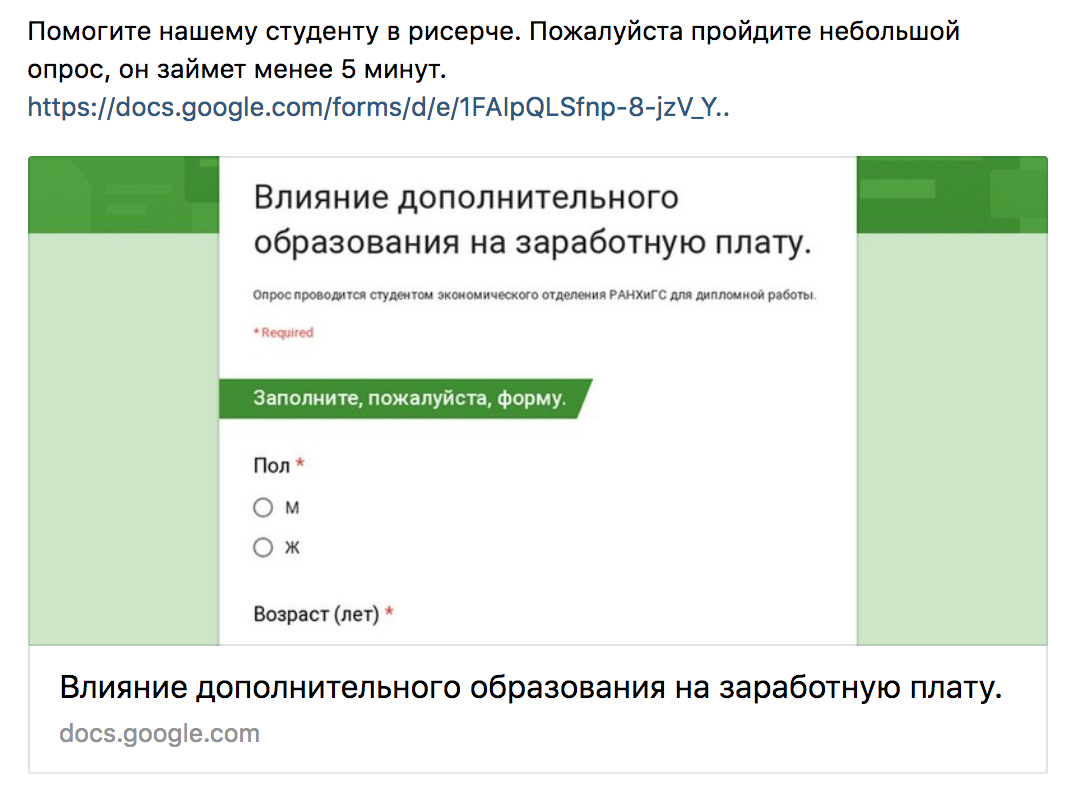
\includegraphics[scale=0.3]{research.png}
\end{center} 
Как считаете, какие проблемы возникнут у исследователя с выборкой? 

\item Радомир ушёл заниматься машинным обучением в крупную ритейл-компанию. Его главная задача в этом полугодии --- оптимизация издержек. Радомиру нужно научиться предсказывать продажи помидоров в разных частях города, чтобы более оптимально заполнять ими торговые точки. 

Очень плохо, когда в магазин привозят слишком много помидоров и они протухают, либо наоборот слишком мало помидоров, и их не хватает людям. 

Радомир с ходу понял, что перед ним задача регрессии и обучил случайны лес. Теперь он умеет предсказывать спрос на помидоры в каждом магазине города в любой день года. Судя по тестовой выборке модель Радомира помогает сэкономить. Как можно было бы убедиться в этом на практике и не поломать продажи? На что надо обратить внимание при дизайне АБ-теста? 
\end{itemize}
\end{problem}

\begin{solution}
\begin{itemize} 
\item Выборка повреждений самолётов в наших руках нерепрезентативна. Самолёты с критическими повреждениями не долетают до аэродрома. Значит нужно укреплять те части самолётов, где пробоин нет. Именно такой совет дал Абрахам Вальд. 

\item Эксперты стали разбираться почему так произошло, ведь в рамках фокус-группы было показано, что больше сахара --- это вкуснее. Выяснилось, что это исследование проходило не в тех самых условиях, в которых люди обычно пьют Кока-Колу. 

Если речь идёт всего лишь об одном стакане, то, действительно, людям нравится большее количество сахара. Однако если напиток употребляется постоянно в больших количествах, то больше сахара --- хуже. Кажется, что это логично: сложно выпить большое количество очень сладкого напитка. Поэтому, когда проводятся исследования на фокус-группах, нужно следить за тем, чтобы условия были максимально приближены к настоящим.

\item Обычно различные продуктовые изменения в компаниях принимают с помощью АБ-теста. В ситуации Радомира нужно выделить из всех пользователей случайный $1\%$ и показать им новую кнопку.  После нужно проверить гипотезу о том, что доля людей, нажавших на новую кнопку никак не оличается от доли людей, которые жали на старую кнопку. 

Если неожиданно окажется, что в долях есть значимое различие, то кнопку и правда можно заменить на новую. 

\item Возникает штука, которая называется проблема самоотбора. Анкету, которая вывешена таким образом, заполнит далеко не каждый человек. Полученная в конечном итоге выборка не будет случайной. Она охватит лишь какой-то конкретный сегмент друзей пользователя.

Более того, заполнение анкеты может само по себе зависеть от какой-то скрытой переменной. Это приведёт к смещённым и несостоятельным результатам даже если удастся выйти за круг друзей и добиться случайного заполнения анкеты. Например, в данном случае маловероятно, что люди с высокой зарплатой решат потратить своё время на заполнение подобной анкеты. Их время слишком дорого стоит. Анкету в основном заполнят безработные студенты, залипающие вконтакте. В конечном итоге, имея в выборке мало примеров людей с высокой зарплатой, мы будем исследовать не совсем то явление, которое собирались исследовать в начале и сделаем некорректные выводы.

\item Мы с вами заходим на страшную территорию АБ-тестирования в оффлайне. Когда мы делаем АБ-тест в интернете, довольно легко выделить случайный $1\%$ людей и на нём проверить свои идеи. 

Если речь идёт о реальных магазинах, которые стоят в реальных городах, мы сталкиваемся с определёнными сложностями. Если действовать по стандартной методологии, Радомиру нужно выделить среди магазинов группу, для которой о начнёт использовать свою модель. Спустя месяц можно будет посмотреть на то, какое число помидоров списывается в разных группах, не испортился ли средний чек по помидорам и другие метрики. Если среди них будет значимое улучшение, то  модель Радомира раскатывается на большее число магазинов. 

Однако в такой схеме при дизайне эксперимента многие вещи могут пойти не так. Например, мы можем выбрать для АБ-теста только те районы, которые обладают какой-то определенной спецификой и не заметить этого: более криминогенные, более богатые, более густонаселенные и тп.

Мы можем запустить тест, и сразу же с его запуском в части районов начнут праздновать <<помидорный спас>> и спрос на них резко вырастет, что загубит эксперимент. 

Может произойти очень много странной ерунды, которую мы не ожидали встретить. Поэтому с оффлайн тестами надо быть вдвойне осторожным. Для них обычно придумывают разные специальные техники проведения. Подробнее про них можно почитать на Хабре \href{https://habr.com/ru/company/X5RetailGroup/blog/466349/}{в статейке от X5RetailGroup.} Ну или в \href{https://habr.com/ru/company/ods/blog/416101/}{статейке от Паши Нестерова.}
\end{itemize}
\end{solution} 


\end{document}


